\documentclass[IN,english]{tumbook}
\usepackage{tabularx}
%\usepackage[utf8]{inputenc}
%\usepackage[T1]{fontenc}
%\usepackage{graphicx}
%\usepackage{amsmath}

\makeindex

% Information for the title page
\Seminar{Software Engineering for Business Applications - Master}
\Semester{SS 2015}
\title{Mockups for the Web Application \emph{Travel Diary}}
\Untertitel{}
\Themensteller{Prof. Dr. Florian Matthes}
\Autorenadresse{}
\Matrikelnummer{}
\Fachsemester{}
\Abgabetermin{13. May 2015}
\author{Chetan Basuray, Mantosh Kumar, Ulrike Niemann, Albert Steckermeier}
\date{13. May 2015}



\begin{document}

\maketitle
\newpage
\tableofcontents
\newpage

\chapter{Use Case 1: Searching for Vacations}

Since we want users to search using keywords, we provide users with keywords for search. Of course, the users may also type in search words, if they so choose. Once the user chooses a particular keyword, we will provide the user with related keywords to choose from. Along with this, we also provide users with search results for the chosen keywords. We can see the keywords searched for in the \emph{Selected keywords} section, also the next possible choices are available to the user for selection. Additionally we also see the search results at the bottom of the screen for the chosen keywords. Also results are shown as per user input. If the user inputs names of sites or activities, then we will show them the cities/places where the user may find those activities. However, if the user just inputs the name of a city, we will only show him whatever activities he or she may be able to find in that city.

\begin{figure}[h]
	\begin{center}
		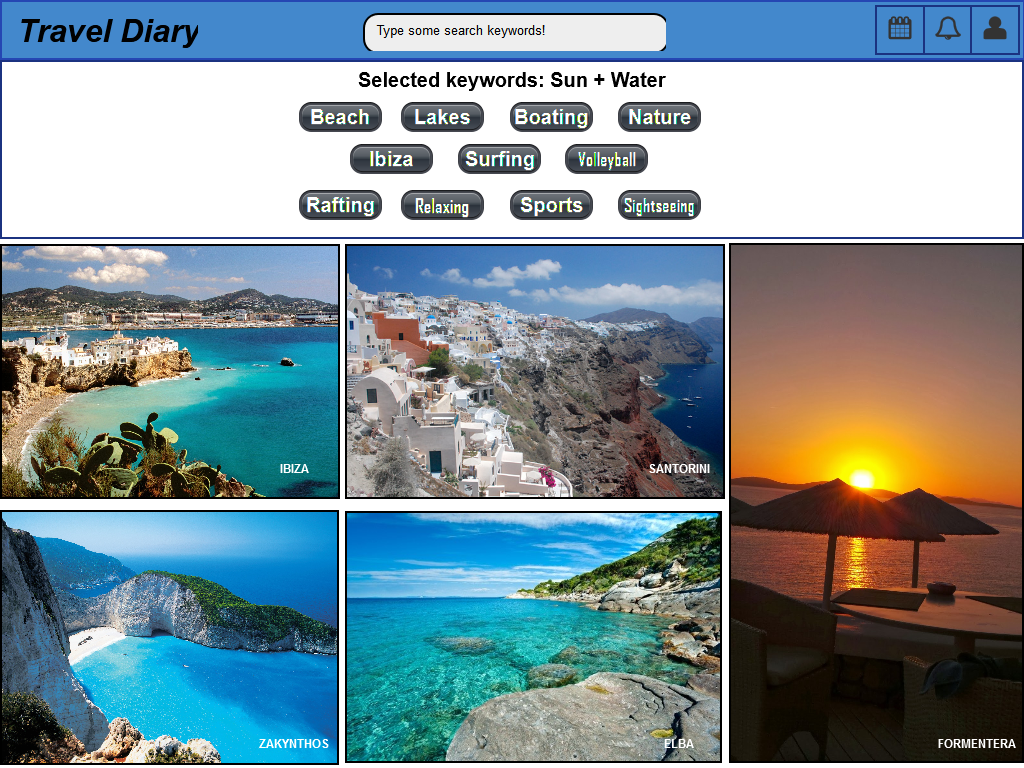
\includegraphics[width=\textwidth]{graphics/usecase1}
	\end{center}
	\label{fig:usecase1}
	\caption{Mockup for the vacation search of \emph{Travel Diary}.}
\end{figure}

\newpage

\chapter{Use Case 2: Sharing the Experience of an Activity}

The web application allows the user to create a private entry about an activity and his experiences in form of a diary. The user can directly add his thoughts about an activity in the trip overview. On mouse-over the view of a single activity expands and gets highlighted. The user now sees a preview of more pictures and by clicking on them he can view them in detail. The user can also upload new images. All images are by default only visible to the user himself. Furthermore existing entries are displayed and new diary entries can be added.

\begin{figure}[h]
	\begin{center}
		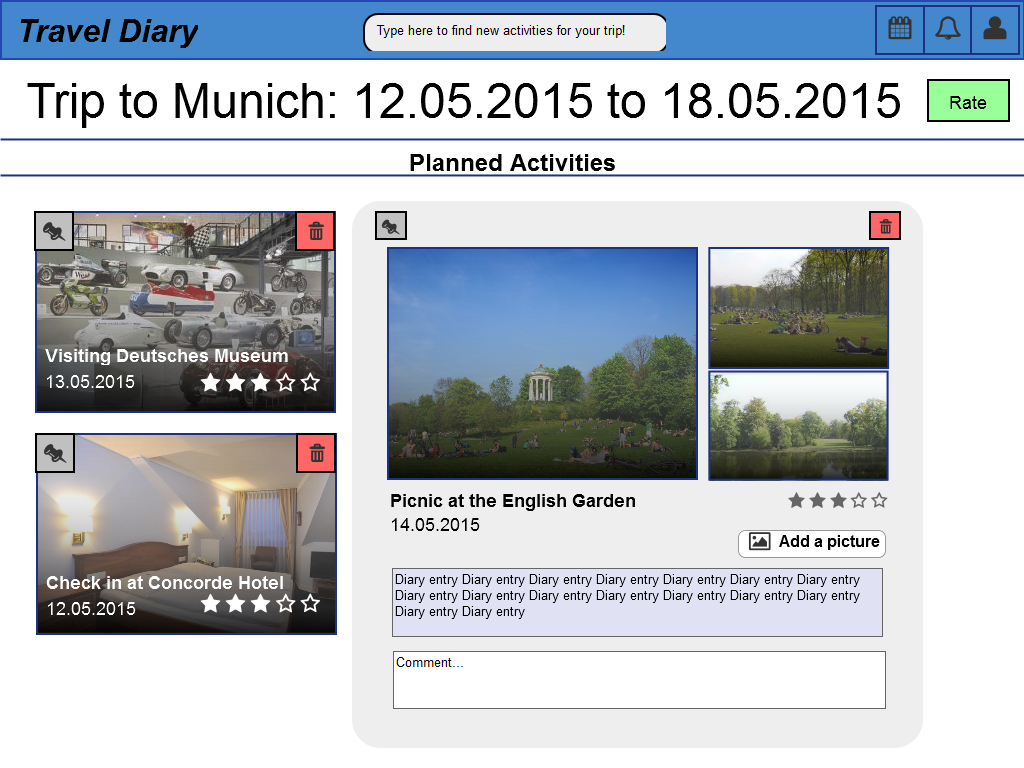
\includegraphics[width=\textwidth]{graphics/usecase2}
	\end{center}
	\label{fig:usecase2}
	\caption{Mockup for sharing the experience of an activity in \emph{Travel Diary}.}
\end{figure}

\newpage

\chapter{Use Case 3: Sharing the Experience of a Vacation}

The link for writing overall experience should be available where user is maintaining his public/private diaries of his vacation. Once he is finished with writing individual reviews (optional) of events, activities and places that he visited then he should be able to add this overall experience. When other user will search and click on some vacation plan in our web app, they can see the the overall experience and individual diary entries of that vacation plan in chronological order.

\begin{figure}[h]
	\begin{center}
		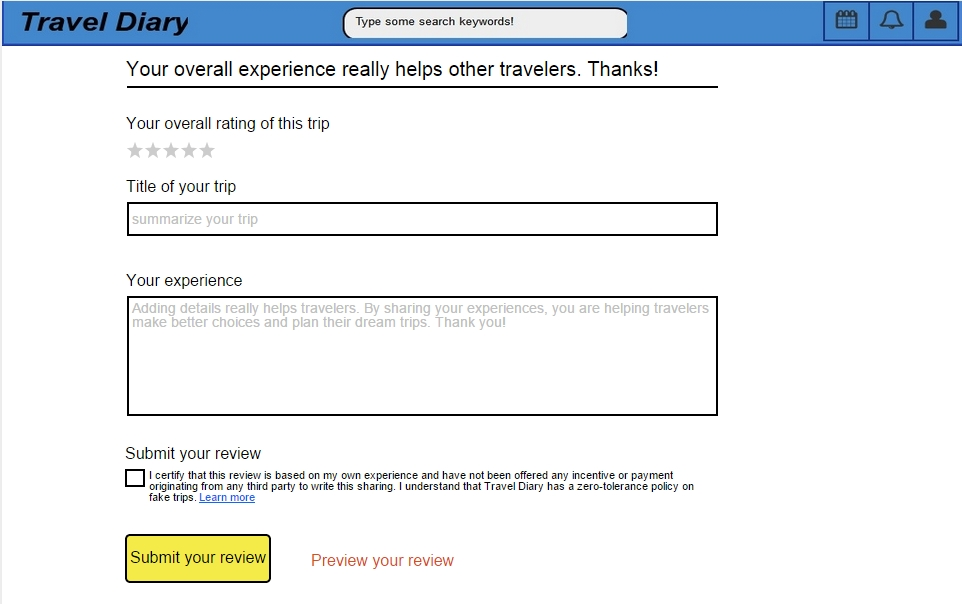
\includegraphics[width=\textwidth]{graphics/usecase3}
	\end{center}
	\label{fig:usecase3}
	\caption{Mockup for sharing the overall experience of a vacation in \emph{Travel Diary}.}
\end{figure}

\newpage

\chapter{Use Case 4: Planning a Vacation}

Figure \ref{fig:usecase4} shows the vacation view. Here all the activities of the vacation \emph{Trip to Munich} are shown. The pin icon at the top left of an activity allows the user to move the activities around. Activities can be deleted by clicking the red trash icon in the top right corner. In the vacation view the search bar at the top automatically searches for activities instead of vacations. A new activity is added by searching it via the search bar and adding it by clicking an add button which will replace the trash icon in the search results for new activities.

\begin{figure}[h]
	\begin{center}
		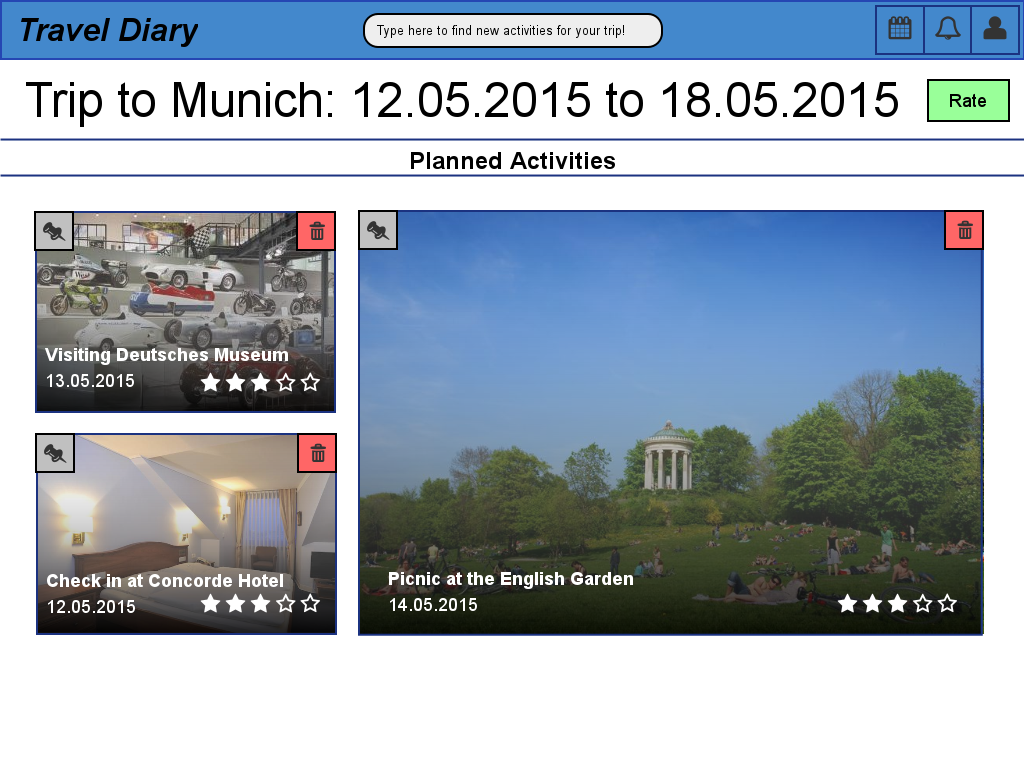
\includegraphics[width=\textwidth]{graphics/usecase4}
	\end{center}
	\label{fig:usecase4}
	\caption{Mockup for the vacation view of \emph{Travel Diary}.}
\end{figure}

\end{document}